\section{Methodology}
This section describes how the speedup-techniques was explored and implemented. Each algorithm was evaluated using the $(9, 2)$, $(11, 3)$, $(13, 4)$, $(15, 5)$ and $(17, 6)$ challenge instances. An $(l, d)$ problem instance is said to be challenging if $d$ is the largest integer value for which the expected number of motifs of lenght $L$ would occur in the input by random chance and does not exceed a constant value (500) \cite{pms2015}.

\begin{figure}[h]
	\centering
	\label{fig:methodology}
	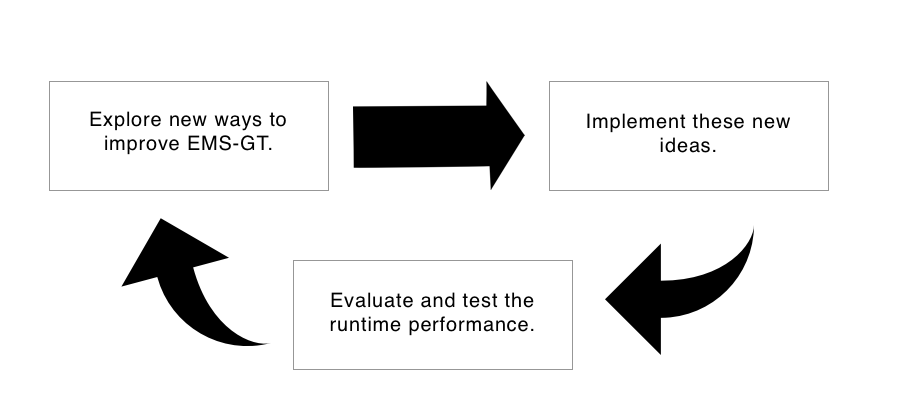
\includegraphics[width=5.5in]{contents/00_images/methodology}
	\caption{Speedup Technique Development Cycle.}
\end{figure} 

The study aims to improve the algorithm by pre-computation of values and exploring other usage of the block-processing technique. The speedup techniques was developed using the development cycle shown in Figure \ref{fig:methodology}.

\subsection{Improving the EMS-GT}
%  C++ implementation
Originally, EMS-GT was implemented using Java, but for the purpose of eliminating variables that may affect the evaluation of the algorithms, it was converted to C++. 

% block flags
A previous study \cite{sia2015} improved the neighborhood generation by setting the search space by blocks instead of one bit at a time. The generation phase quickly filters the search space as it process the neighborhood of the sequence, leaving numerous empty blocks of $l$-mers in the candidate motifs array. It was observed that at some point in the generation phase, some of the block settings are not necessary anymore since that block is already empty in the candidate motifs array. We improved the algorithm by maintaining boolean flags for those empty blocks. Then we ignore all block bit settings for those empty blocks.

% faster candidate motif elimination
Additionally, the block-processing procedure was found useful in the testing of candidate motifs. Grouping the candidate motifs by blocks 

% pre computation

% n' values then parameter fine tuning




